\documentclass[a4paper, 11pt]{article}

\usepackage[absolute]{textpos} % absolute positioned text blocks
\setlength{\TPHorizModule}{1mm}
\setlength{\TPVertModule}{1mm}
\usepackage[english]{babel}
\usepackage{csquotes}

% Images
\usepackage{graphicx} % used for images
\graphicspath{ {./img/} }
\usepackage[labelfont=bf]{caption}

% Formatting
\usepackage{geometry} % better margins for document
\usepackage{titlesec} % better control over title spacing 
\usepackage{tabularx} % better tables
\usepackage[hidelinks]{hyperref} % hrefs
\usepackage{totcount}

% Gantt charts
\usepackage{pgfgantt}
\usepackage{float}

\geometry{
	a4paper,
	left=28mm,
	right=28mm,
    top=30mm,
    bottom=30mm
}

% Colors 
\RequirePackage{color}
\definecolor{bfhgrey}{rgb}{0.41,0.49,0.57}

% Glossary
\usepackage[toc]{glossaries}
% Acronyms
\newglossaryentry{hlsl}{name={HLSL}, text={HLSL}, first={high-level shading language (HLSL)}, description={High-level shading language. Developed by microsoft, this is a standard shader language for DirectX used in graphics programming}}
\newglossaryentry{json}{name={JSON}, text={JSON}, first={Java-Script object notation (JSON)}, description={Java-Script object notation. A light-weight data format that is stored as human-readable text}}
\newglossaryentry{slpk}{name={SLPK}, text={SLPK}, first={ESRI scene layer package (SLPK)}, description={ESRI scene layer package A custom, web-optimized format used for files related to ESRI }}
\newglossaryentry{png}{name={PNG}, text={PNG}, first={portable network graphic (PNG)}, description={Portable network graphic. A common format for lossless compressed image files}}
\newglossaryentry{ui}{name={UI}, text={UI}, first={user interface (UI)}, description={User interface. The interface that allows the user to interact with the software}}
\newglossaryentry{gpu}{name={GPU}, text={GPU}, first={GPU}, description={Graphics processing unit. A piece of hardware designed to rapidly manipulate and alter memory, often intented for output to a display device}}
\newglossaryentry{wmo}{name={WMO}, text={WMO}, first={World Meteorological Organization (WMO)}, description={A specialized agency conducting atmospheric science, climatology, hydrology and geophysics}}

% Glossary entries
\newglossaryentry{latex}{name=LaTeX, description={ A high-quality document preparation system designed for the production of technical and scientific documentation }}
\newglossaryentry{noisegeneration}{name=Noise generation, text={noise generation}, description={ Noise generation is used to generate textures of one or more dimension with seemingly random smooth transitions from black to white (zero to one) }}
\newglossaryentry{volumetric}{name=Volumetric, text={volumetric}, description={ This describes a technique which takes a 3D volume of data and projects it to 2D. It is mostly used for transparent effects stored as a 3D image }}
\newglossaryentry{raymarching}{name=Ray marching, text={ray marching}, description={ Ray marching is a type of method to approximate the surface distance of a volumetric object, where a ray is cast into the volume and stepped forward until the surface is reached }}
\newglossaryentry{lightmarching}{name=Lightmarching, text={lightmarching}, description={ The same concept as \gls{raymarching}, but instead of being cast into the volume, it is cast towards the primary light source with a constant step }}
\newglossaryentry{billboard}{name=Billboard, text={billboard}, description={ A 2D image always facing towards the main camera }}
\newglossaryentry{worldspace}{name=World space, text={world space}, description={ Coordinates defined with respect to a global Cartesian coordinate system }}
\newglossaryentry{polymesh}{name=Polymesh, text={polymesh}, description={ A polymesh is a 3D model composed of polygons or triangles }}
\newglossaryentry{lowpoly}{name=Low poly, text={low poly}, description={ A 3D polymesh with a relatively low count of polygons }}
\newglossaryentry{voxel}{name=Voxel, text={voxel}, description= { Short for \textit{volume element}, a voxel is a value (either a number or a vector) on a scalar or vector field }}
\newglossaryentry{scalarfield}{name=Scalar field, text={scalar field}, description={ A scalar field describes a typically three-dimensional grid of elements called \textit{voxels}, each containing a scalar value }}
\newglossaryentry{vectorfield}{name=Vector field, text={vector field}, description={ It is the same as a scalar field, except the voxels are vector values }}
\newglossaryentry{spheretracing}{name=Sphere tracing, text={sphere tracing}, description={ Sphere tracing describes an optimized algorithm of ray marching by using signed distance functions to approximate the surface distance of the volume }}
\newglossaryentry{sdf}{name=Signed distance function, text={signed distance function}, description={ A signed distance function, short SDF, returns a positive distance if the origin is outside the volume and a negative distance if it is inside the volume }}
\newglossaryentry{surfacenormal}{name=Surface normal, text={surface normal}, description={ A \textit{surface normal} or \textit{normal} is a vector which is perpendicular to a given geometry, like a triangle or polygon }}
\newglossaryentry{gradient}{name=Gradient, text={gradient}, description={ The \textit{gradient} denotes the direction of the greatest change of a scalar function }}
\newglossaryentry{penumbra}{name=Penumbra, text={penumbra}, description={ The partially shaded outer region of diffuse shadows. Also described as soft edges }}
\newglossaryentry{shapeblending}{name=Shape blending, text={shape blending}, description={ In SDFs, shapes can be seemingly blended together by returning a interpolated value of those distances }}
\newglossaryentry{ambientocclusion}{name=Ambient occlusion, text={ambient occlusion}, description={ Also known as contact shadows, this method darkens points in the scene that are not or only slightly exposed to the light and its environment }}
\newglossaryentry{noise}{name=Noise, text={noise}, description={ A randomly generated pattern, referring to \gls{procedural} pattern generation }}
\newglossaryentry{translucent}{name=Translucent, text={translucent}, description={ An object or substance that is translucent allows light to be passed through it, meaning it is rendered transparently to some degree }} 
\newglossaryentry{parameters}{name=Parameters, text={parameters}, description={ Shader variables exposed to the Unity Editor }} 
\newglossaryentry{sss}{name=Subsurface scattering, text={subsurface scattering}, description={ SSS is a mechanism of light transport in which light enters a translucent object, is scattered around and exits the material at a different point, resulting in illuminated areas where the material is thin }} 
\newglossaryentry{sunlightforwarding}{name=Sunlight forward scattering, text={sunlight forward scattering}, description={ The process of sunlight shining through and illuminating the clouds which cover the sun }} 
\newglossaryentry{sunlighttransmittance}{name=Sunlight transmittance, text={sunlight transmittance}, description={ In this matter, the same as \gls{sunlightforwarding} }} 
\newglossaryentry{cnn}{name=Convolutional neural network, text={convolutional neural network}, description={ A neural network that is able to classify images }} 
\newglossaryentry{gan}{name=Generative adverserial network, text={generative adverserial network}, description={ A set of two neural networks, where one generates images and the other tries to tell wether those images are real or generated }} 
\newglossaryentry{aabb}{name=Axis-aligned bounding box, text={axis-aligned bounding box}, description={ A non-rotated bounding box enclosing an object completely }} 
\newglossaryentry{shader}{name=Shader, text={shader}, description={ A piece of software which runs on the \gls{gpu}, rendering geometrically defined objects to the screen  }} 
\newglossaryentry{computeshader}{name=Compute shader, text={compute shader}, description={ A shader which runs on the GPU but outside of the default render pipeline }} 
\newglossaryentry{fbm}{name=Fractal Brownian motion, text={fractal Brownian motion}, description={ Different iterations of continuously more detailed noise layered on top of each other }} 
\newglossaryentry{fractalnoise}{name=Fractal noise, text={fractal noise}, description={ In this matter, the same as \gls{fbm} }} 
\newglossaryentry{procedural}{name=Procedural, text={procedural}, description={ Created solely with algorithms and independant of any prerequisites }}
\newglossaryentry{histogram}{name=Histogram, text={histogram}, description={ A graphical representation of data like brightness or color distribution of a given photograph }}
\newglossaryentry{csg}{name=Constructive solid geometry, text={constructive solid geometry}, description={ Short CSG, stands for combining primitive geometric objects with Boolean operators }}
\newglossaryentry{neuralnetwork}{name=Neural network, text={neural network}, description={ A series of algorithms that can recognize and categorize certain patterns in a given set of data }}
\newglossaryentry{interpolation}{name=Interpolation, text={interpolation}, description={ In mathematics, interpolation describes a method of estimating unknown values that fall between known values }}
\newglossaryentry{wrs}{name=Weather rendering system, text={weather rendering system}, description={ The Unity application that is implemented during this project. It takes in live data from a weather service and uses topological elevation models to create a weather simulation, which is then rendered and up for comparison with live photographs }}
\newglossaryentry{altitude}{name=Altitude, text={altitude}, description={ A vertical distance measurement, in this context specifically the distance from sea level to the given object }}
\newglossaryentry{watervapor}{name=Water vapor, text={water vapor}, description={ Evaporated water in a gaseous form }}
\newglossaryentry{desublimation}{name=Desublimation, text={desublimation}, description={ The process of gas transitioning to liquid without passing through the liquid phase }}
\newglossaryentry{halophenomenon}{name=Halo phenomenon, text={halo phenomenon}, description={ White or colored rings or arcs of light around the sun or the moon, produced by cirrostratus clouds }}
\newglossaryentry{cloudlet}{name=Cloudlet, text={cloudlet}, description={ Small, white, puffy clouds that come in large quantities, together forming a cloud of the cumulus family }}
\newglossaryentry{precipitation}{name=Precipitation, text={precipitation}, description={ Rainfall. The result of atmospheric water vapor that has been condensed and now falls from clouds }}
\newglossaryentry{convection}{name=Convection, text={convection}, description={ The process of warm air rising from the surface and cooling at higher altitude, of which the moisture is then condensed into clouds }}
\newglossaryentry{thermal}{name=Thermal, text={thermal}, description={ In relation with meteorology, the hot, rising air from convection is called "thermal" }}
\newglossaryentry{weatherfront}{name=Weather front, text={weather front}, description={ A boundary between to air masses, which differ in temperature, wind direction and humidity }}
\newglossaryentry{warmfront}{name=Warm front, text={warm front}, description={ A warm \gls{weatherfront}, the boundary of a mass of air that carries mild or warm air. When colliding with a \gls{coldfront}, \gls{precipitation} is often followed }}
\newglossaryentry{coldfront}{name=Cold front, text={cold front}, description={ A cold \gls{weatherfront}, the boundary of a mass of air that carries cold or cool air. When colliding with a \gls{warmfront}, \gls{precipitation} is often followed }}
\newglossaryentry{occludedfront}{name=Occluded front, text={occluded front}, description={ When a cold front overtakes a warm front, it pushes the warm air upwards (\gls{thermal}s). The moisture of the warm air condenses as it rises, creating \gls{watervapor}. This often results in clouds with \gls{precipitation} }}
\newglossaryentry{occlusion}{name=Occlusion, text={occlusion}, description={ In meteorology, the clash of a warm front and a cold front. See \gls{occludedfront} }}
\newglossaryentry{lerp}{name=Linear interpolation, text={linear interpolation}, description={ Simply put, linear interpolation describes a method of finding values inbetween two points on the same line }}
\newglossaryentry{particlesystem}{name=Particle system, text={particle system}, description={ In computer graphics, a particle system is a technique that continuously spawns and recycles objects. They are often used to reproduce fire or smoke effects, with small flame or dust textures as particles }}
\newglossaryentry{pseudorandom}{name=Pseudo-random, text={pseudo-random}, description={ A random number generated with a deterministic algorithm, meaning that the same input will always give the same output }}
\newglossaryentry{textureslice}{name=Texture slice, text={texture slice}, description={ A 2D texture extracted from a 3D texture for a given depth }}

\makenoidxglossaries

% Bibliography
\usepackage[backend=biber, style=ieee]{biblatex}
\addbibresource{partials/specification.bib}

\begin{document}

\color{black}

\title{\doctitle}
\author{\docauthor}
\date{\versiondate} 

\newcounter{requirements}
\newcounter{testcases}
\newtotcounter{versionnumber}
\newcommand{\docsubtitle}{Requirements Specification}
\newcommand{\docauthor}{Matthias Thomann}
\newcommand{\doctitle}{Real-time Weather Rendering System}
\newcommand{\fieldofstudies}{BSc in Computer Science}
\newcommand{\specialisation}{Computer perception and virtual reality}
\newcommand{\prof}{Prof. Urs K\"unzler}

\newcommand{\versiondate}{\today}
\newcommand{\sectionref}[1]{\autoref{#1}}
\newcommand{\emptyline}{\vspace{\baselineskip}\\\noindent}

\titlespacing*{\section} {0pt}{7.5ex plus 1ex minus .2ex}{2.3ex plus .2ex}
\titlespacing*{\subsection} {0pt}{4.25ex plus 1ex minus .2ex}{1.5ex plus .2ex}

\pagenumbering{roman}
\setcounter{page}{3}

%% include BFH logo and HuCE-ml logo

\begin{titlepage}

\setlength{\unitlength}{1mm}

\begin{textblock}{20}[0,0](22,12)
    
\includegraphics{../img/BFH_Logo_B.png}
\end{textblock}

\begin{flushleft}

\vspace*{21mm}

\fontsize{24.88pt}{40pt}\selectfont
\textbf{\doctitle}
\vspace{2mm} 

\fontsize{17.28pt}{24pt}\selectfont\vspace{0.3em}
\docsubtitle
\vspace{6mm}

\begin{figure}[H]
    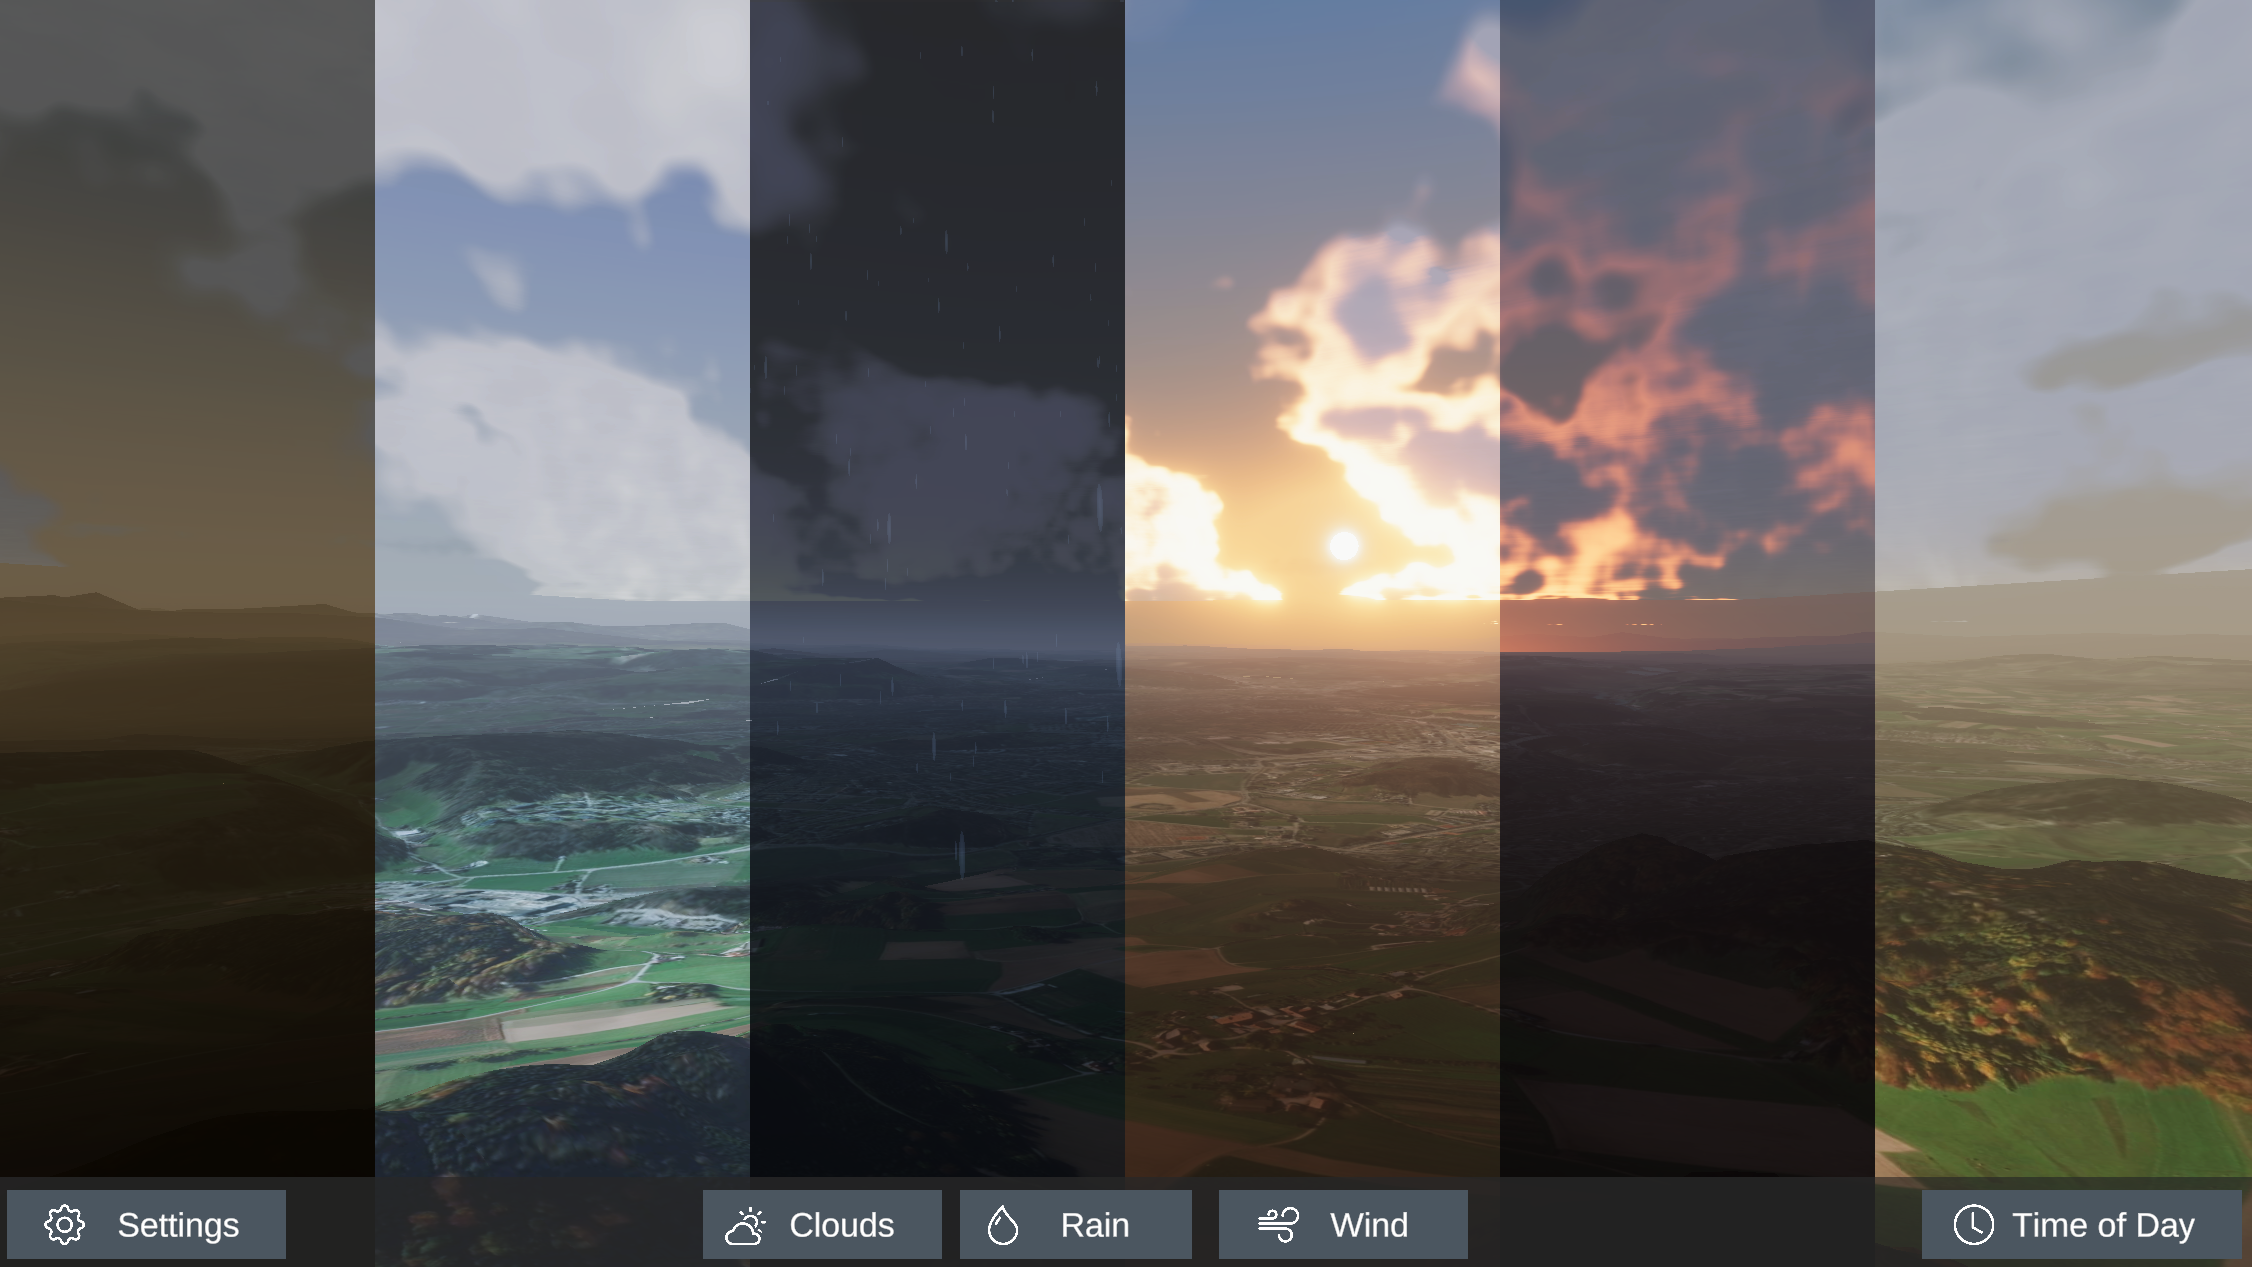
\includegraphics[width=\linewidth]{results/wheel.png}
\end{figure}

\fontsize{10pt}{12pt}\selectfont
\begin{textblock}{150}(28,225)
\begin{tabbing}
xxxxxxxxxxxxxxxxxxxxx\=xxxxxxxxxxxxxxxxxxxxxxxxxxxxxxxxxxxxxxxxxxxxxxx \kill
Field of Studies:	\> \fieldofstudies	\\
Specialization:	    \> \specialisation	\\
Author:		        \> \docauthor \\
Supervisor:         \> \prof \\
Date:			    \> \versiondate \\
Version:		    \> 1.0 \\
\end{tabbing}

\end{textblock}

\begin{textblock}{150}(28,280)
\noindent 
\color{bfhgrey}\fontsize{9pt}{10pt}\selectfont
Berner Fachhochschule | Haute \'ecole sp\'ecialis\'ee bernoise | Bern University of Applied Sciences
\color{black}\selectfont
\end{textblock}

\end{flushleft}

\end{titlepage}

\tableofcontents 
\clearpage

\pagenumbering{arabic}

\section{General}

\subsection{Purpose}
This document serves the purpose of defining and clarifying the goals, which the thesis 'Realtime Weather Rendering System' is supposed to achieve. Furthermore, the requirement specification allows for a more accurate evaluation of the achievement of objectives and of the result itself.

\subsection{Revision History}
\begin{tabularx}{\textwidth}{|l|l|l|X|}
    \hline
    \textbf{Version}         & \textbf{Date}        & \textbf{Name}     & \textbf{Comment}                  \\ \hline \addtocounter{versionnumber}{1}
    0.\arabic{versionnumber} & February 27, 2021    & Matthias Thomann  & Initial draft                     \\ \hline \addtocounter{versionnumber}{1}
    0.\arabic{versionnumber} & March 03, 2021       & Matthias Thomann  & Updated project schedule          \\ \hline
\end{tabularx}
\clearpage

\section{Vision}

\subsection{Weather Rendering System}
This section defines a high-level vision for the desired outcome of this thesis and potential future work.
As listed in the primary goals, the weather rendering system will be based on compute shaders.
Compared to the prototype from the previous project, this is expected to result in a much better performance.
That in turn, allows for a more complex and realistic model.
\\
With the incorporation of real-time weather data and the use of topological landscape data, any given weather scenario could be simulated and rendered.
The desired outcome ideally looks similar to the image depicted in \autoref{img:rendered1}.
A rendered version of such a cloud system can look elusively realistic compared to an actual photograph, like in \autoref{img:photo1}.
\begin{figure}[ht]
    \centering
        \begin{minipage}{0.47\linewidth}
            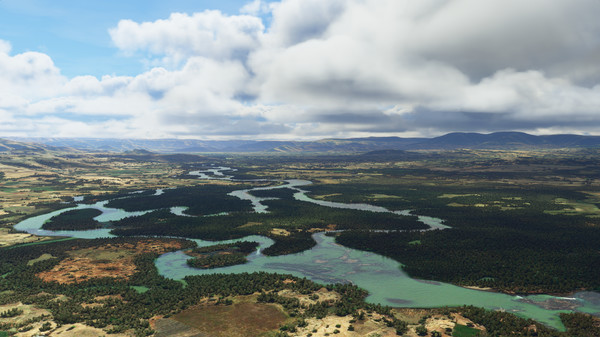
\includegraphics[width=\linewidth]{msfs-ref1.jpg}
            \captionof{figure}{A rendered image of volumetric clouds \protect\cite{img:rendered:clouds01}.}
            \label{img:rendered1}
        \end{minipage}
    \hfill
        \begin{minipage}{0.47\linewidth}
            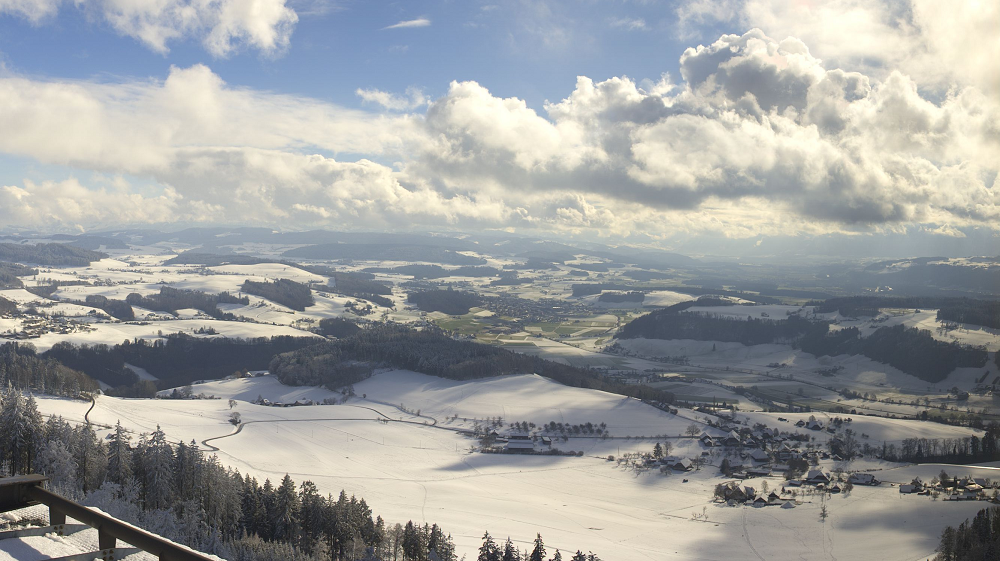
\includegraphics[width=\linewidth]{roundshot2021-01-18-12-50-cropped.png}
            \captionof{figure}{A photographic reference of clouds \protect\cite{img:photo:clouds01}.}
            \label{img:photo1}        
        \end{minipage}  
\end{figure}
\\
The first thought about the practical use of a fully-fledged volumetric cloud system might be a video game, since clouds are often a significant part of outdoor scenery in games.
However, for this thesis it is intended that the knowledge and results acquired during the given period will be used to recreate a lifelike weather system instead.

\clearpage

\subsection{System Overview}
To get a better understanding of how such a system could be implemented, this diagram shows all the involved components and their processes.
\begin{figure}[H]
    \centering
    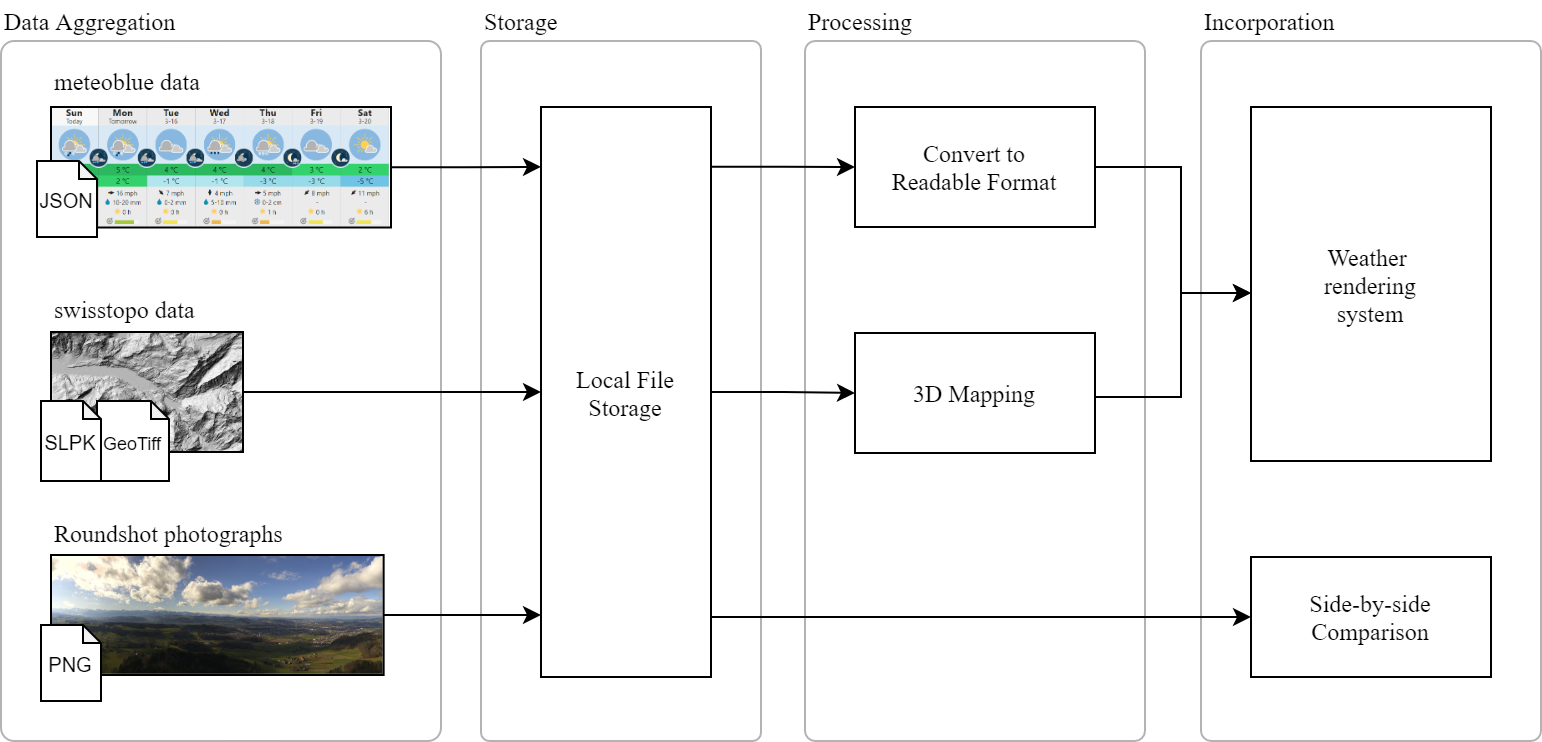
\includegraphics[width=\linewidth]{system diagram.png}
    \captionof{figure}{System overview diagram.}
    \label{img:systemoverview}
\end{figure}

\noindent
All external data is retrieved regularly and stored on the local file system. Their respective file formats are denoted in the bottom left corner of each data source.
After aggregation, the data is processed into a readable and compatible format for the Unity Engine. From there, the weather rendering system can make unrestricted use of the data.
The resulting output of the system can then be compared side-by-side with the collected real-life photographs.

\subsection{External Data}
\subsubsection{Meteoblue Weather Data}
To accurately reflect a weather system, conditions like precipitation, wind and cloudiness will be considered.
Fortunately, the company \emph{meteoblue} offers this data in form of different data packages \cite{meteoblue}.
As an additional bonus, the license costs are drastically reduced for student projects and educational work.
\\
From all available data packages, the "basic\textunderscore1h" \cite{meteoblue:basic1h} offer seems the most fitting for this thesis.
It includes the most common weather variables only, but this will clearly suffice for the planned project.
Some of the crucial variables are wind speed, wind direction, temperature, sea level pressure, and a pictocode.
\\
The weather data will be requested for the following locations:
\begin{itemize}
    \item Bern, Switzerland
    \item Fribourg, Switzerland \\(to account for the weather in the background of the photographs)
    \item Solothurn, Switzerland \\(to account for the weather in the background of the photographs)
\end{itemize}

\noindent
This data is retrieved on a daily basis and stored on a local file system for the duration of the thesis. The file format is \gls{json}.

\subsubsection{Roundshot Photographs}
The weather data from \emph{meteoblue} gives detailed information about the weather at a specific time and date.
But to be able to compare the rendered result of the weather system with the actual weather of that period, real photographs of the same time should be used.
That is why images taken by the \emph{Roundshot} camera system from the company \emph{Seitz} \cite{roundshot} are stored periodically.
\\
There are many installations of those systems across the country. For this project, the following two locations are used: 
\begin{itemize}
    \item Roundshot camera Bantiger, Switzerland \cite{bantiger}
    \item Roundshot camera Gurtenpark, Switzerland \cite{gurtenpark}
\end{itemize}

\noindent
This data is retrieved on a weekly basis and stored on a local file system for the duration of the thesis. The file format is \gls{png}.

\subsubsection{Swisstopo Height Models}
The last part of a convincing weather rendering system is the landscape. For that, the topologically accurate 3D height model data from the company \emph{swisstopo} will be used \cite{swisstopo}.
As of March 2021, \emph{swisstopo}'s height models and landscape data are available free of charge \cite{swisstopo:free}.
The goal is to download and convert this data into a Unity-compatible 3D model and use it as a base for the scenery.

\noindent
This data is retrieved once or whenever an update is due and stored on a local file system for the duration of the thesis. The file format is \gls{slpk} or any othersuitable data format by the company ESRI.

\clearpage

\subsection{UI Mockup}
As for the \gls{ui}, there will be two possible modes to choose from.
The first one is a "real-life" mode that lets the user choose time and date, for which the weather is then recreated with the \emph{meteoblue} data from that period.
The other mode will be a sandbox mode, where all influencial weather variables can be controlled manually.
\\
The following mockups only serve as a general guideline and are not final.

\begin{figure}[H]
    \centering
    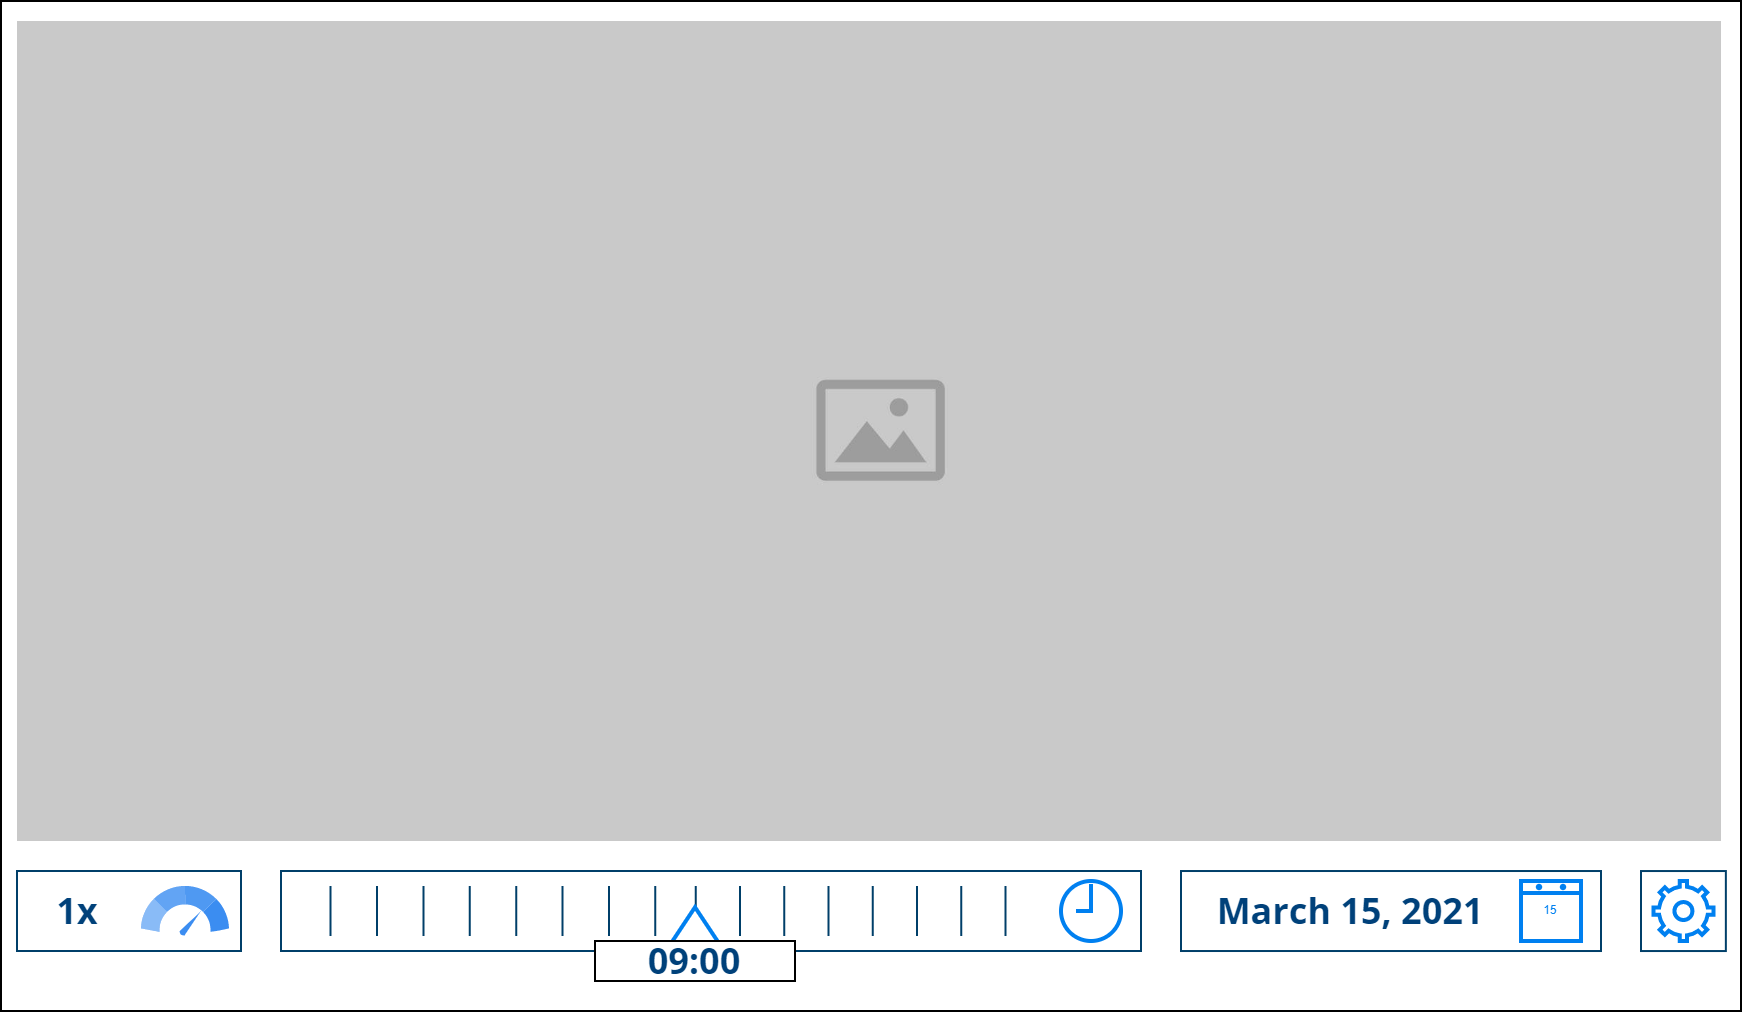
\includegraphics[width=\linewidth]{ui mockup live.png}
    \captionof{figure}{UI mockup of the "real-life" mode.}
    \label{img:ui:mockup:live}
\end{figure}

\begin{figure}[H]
    \centering
    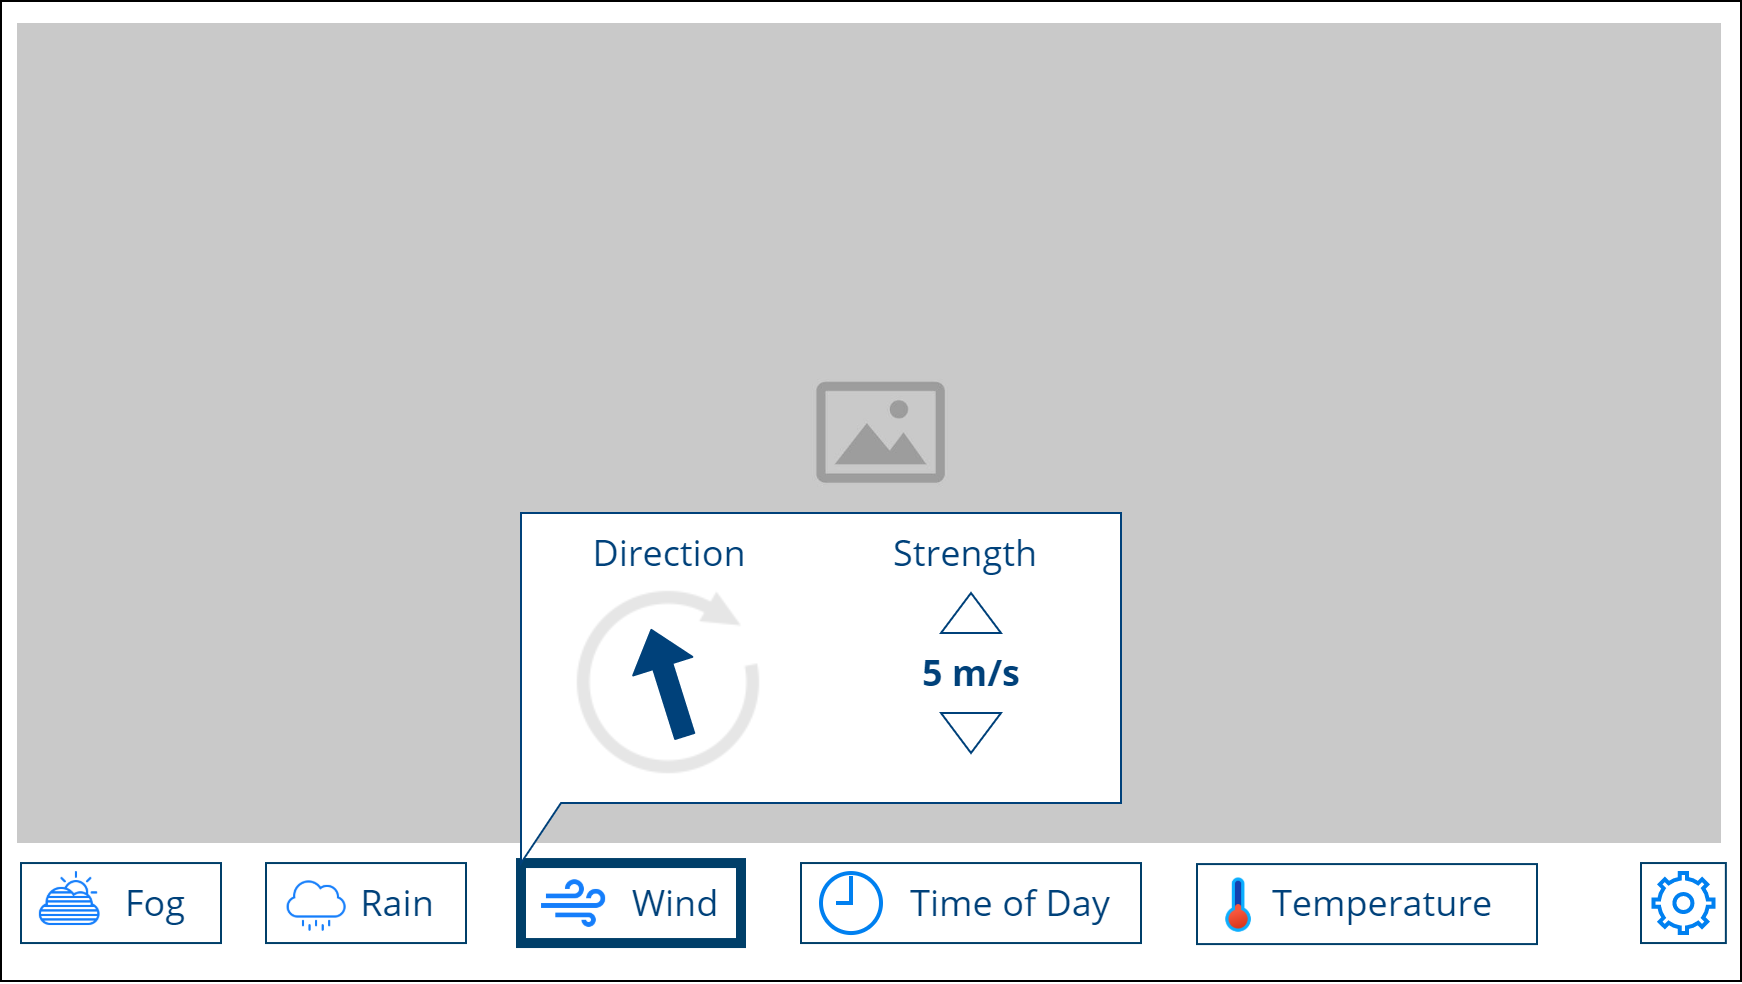
\includegraphics[width=\linewidth]{ui mockup sandbox.png}
    \captionof{figure}{UI mockup of the "sandbox" mode.}
    \label{img:ui:mockup:sandbox}
\end{figure}

\subsection{Future Work}
In a future project, the weather system could evolve into a complete flight simulation game where the player cruises through the clouds, like in Microsoft's \emph{Flight Simulator}.
Another interesting idea is to expand the system into a whole ecosystem with living creatures and animals. Their behaviour would be weather-dependent, making it one big symbiotic environment.
\clearpage

\section{Scope of Work}

\subsection{Initial Situation}
In computer graphics, especially in games, an astonishingly large group of features are reccurring across all programs and genres.
With the most obvious ones being water surfaces, cloudscapes and fire effects, they are present in almost any game. 
Naturally, those features grew in complexity, customizability and computational demands over time.
\\
One of the core mechanics for achieving realistic results is called a \emph{\gls{volumetric} \gls{shader}}.
A prototype such a \gls{shader} has been created in a previous project and will be used as base.

\subsubsection{Previous Work}
In a previous project, the process of creating a \gls{volumetric} \gls{shader} has already been researched and implemented in a prototype. Thanks to its high flexibility, different cloudscapes could be rendered by the same shader.

\begin{figure}[ht]
    \centering
        \begin{minipage}{0.47\linewidth}
            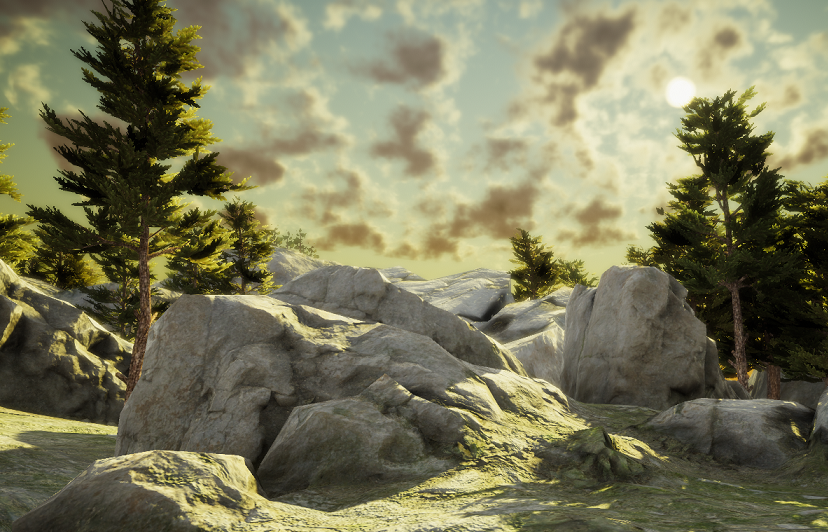
\includegraphics[width=\linewidth]{project2/project2-final.PNG}
            \captionof{figure}{Result of the previous work's shader (Evening).}
        \end{minipage}
    \hfill
        \begin{minipage}{0.47\linewidth}
            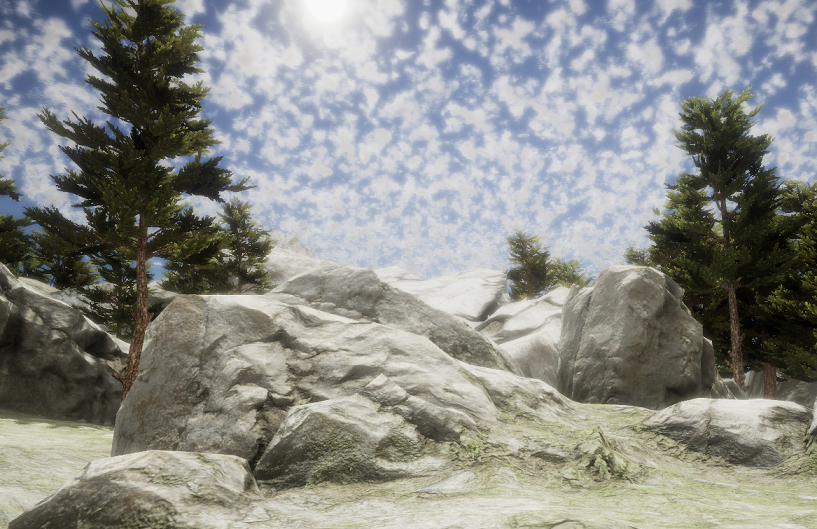
\includegraphics[width=\linewidth]{project2/project2-final2.PNG}
            \captionof{figure}{Result of the previous work's shader (Day).}
        \end{minipage}  
\end{figure}

\noindent
During that project, some other important topics have been researched. Among those were \gls{volumetric} rendering, Perlin and Voronoi \gls{noisegeneration} algorithms, and a technique called \emph{\gls{raymarching}}.
\\
The implementations of those algorithms and methods will most likely be reused in this thesis and will be adapted and improved accordingly.

 \subsection{Goals}
\label{section:goals}
As the title of the thesis suggests, this work will primarily focus on clouds and cloudscapes.
The primary goal of the project is to research and implement rendering techniques for a real-time \gls{procedural} weather rendering system.
\\
The goals will be split into two distinct groups: mandatory and optional. However, this section only defines high-level goals. A detailed specification of all requirements can be found in \sectionref{section:requirements}.

\subsubsection{Mandatory Goals}
The following tasks must be accomplished during the project:
\begin{itemize}
    \item Understanding of different layers of clouds
    \item Understanding of compute shaders
    \item Implement a weather rendering system
    \item Incorporate real-time weather data from \emph{meteoblue}
\end{itemize}

\subsubsection{Optional Goals}
For further optional work, these tasks can be looked into:
\begin{itemize}
    \item Incorporate topological landscape models from \emph{swisstopo}
    \item Automatic validation of realism of rendered cloudscapes
    \item Automatic comparison of rendered cloudscapes and photographs
    \item Automatic categorization of rendered cloudscapes
    \item Performance optimization
\end{itemize}

\clearpage

\subsection{Vision}
This section defines a high-level vision for future work involving the results and implementations of this thesis. 
As listed in the primary goals, the weather rendering system will be based on compute shaders.
Compared to the prototype from the previous project, this is expected to result in a much better performance.
That in turn, allows for a more complex and realistic model.
\\
With the incorporation of real-time weather data and the use of topological landscape data, any given weather scenario could be simulated and rendered.
The desired outcome ideally looks similar to the image depicted in \autoref{img:rendered1}.
A rendered version of such a cloud system can look elusively realistic compared to an actual photograph, like in \autoref{img:photo1}.
\begin{figure}[ht]
    \centering
        \begin{minipage}{0.47\linewidth}
            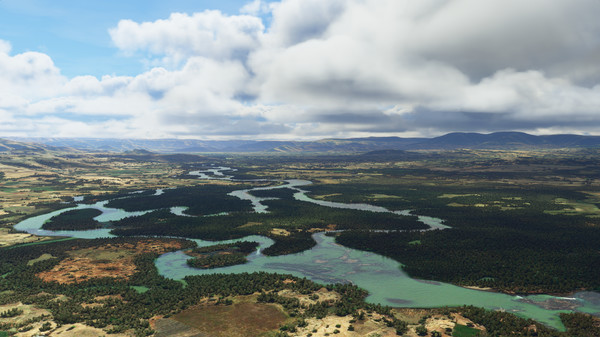
\includegraphics[width=\linewidth]{msfs-ref1.jpg}
            \captionof{figure}{A rendered image of volumetric clouds \protect\cite{img:rendered:clouds01}.}
            \label{img:rendered1}
        \end{minipage}
    \hfill
        \begin{minipage}{0.47\linewidth}
            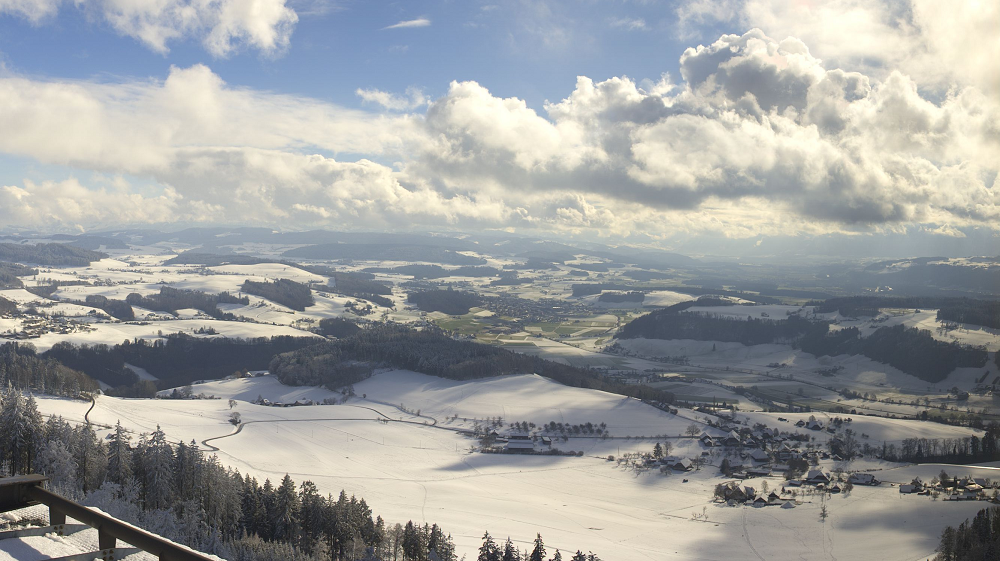
\includegraphics[width=\linewidth]{roundshot2021-01-18-12-50-cropped.png}
            \captionof{figure}{A photographic reference of clouds \protect\cite{img:photo:clouds01}.}
            \label{img:photo1}        
        \end{minipage}  
\end{figure}
\\
The first thought about the practical use of a fully-fledged volumetric cloud system might be a video game, since clouds are often a significant part of outdoor scenery in games.
However, for this thesis it is intended that the knowledge and results acquired during the given period will be used to recreate a lifelike weather system instead.
\\
To accurately reflect a weather system, conditions like precipitation, wind and cloudiness will be considered. This data is obtained from the firm \emph{meteoblue}.

\subsection{Educational Objectives}
Educational objectives include \gls{shader} programming, knowledge about \gls{computeshader}s, rendering techniques, common algorithms used in computer graphics like \gls{noisegeneration}, a general understanding of aspects needed to create a complete weather system and finally the incorporation of real-time data from a third party.

\subsection{Used Software and Tools}
All documentation will be written in \gls{latex} with Visual Studio Code.
The \gls{shader} will be implemented in Unity. The chosen \gls{shader} language is \gls{hlsl}.
For the presentation, Microsoft PowerPoint will be used.
\clearpage

\section{Requirements}
\label{section:requirements}
All requirements are grouped by type. This results in two major groups, which are research and development requirements. Each one of the requirements is derived from a goal listed in \sectionref{section:goals}.

\subsection{Research requirements}
Each research requirement is denoted with the letter "R" followed by its number. They are sorted according to priority, from most important to least important.
\emptyline
\noindent\begin{tabularx}{\textwidth}{|l|X|}
    \hline
    \textbf{Number}     & R.\stepcounter{requirements}\arabic{requirements} \\ \hline
    \textbf{Name}       & Understanding the basic nature of clouds \\ \hline
    \textbf{Description}& In order to be able to recreate a realistically looking cloud shape, one has to examine and understand the way a cloud forms and disperses again first. \\ \hline
\end{tabularx}
\vspace{0.8cm}

\noindent\begin{tabularx}{\textwidth}{|l|X|}
    \hline
    \textbf{Number}     & R.\stepcounter{requirements}\arabic{requirements} \\ \hline
    \textbf{Name}       & Understanding of different layers of clouds \\ \hline
    \textbf{Description}& Among other characteristics, altitude, humidity and atmospheric pressure dictate the look and genus of a cloud. The goal is to decide which cloud types are required for a believable weather system. \\ \hline
\end{tabularx}
\vspace{0.8cm}

\noindent\begin{tabularx}{\linewidth}{|l|X|}
    \hline
    \textbf{Number}     & R.\stepcounter{requirements}\arabic{requirements} \\ \hline
    \textbf{Name}       & Understanding of compute shaders \\ \hline
    \textbf{Description}& Compute shaders proved to be a highly efficient tool when it comes to heavy calculations, like simulations. 
                          To improve performance and therefore allow for more a sophisticated weather system, compute shaders have to be researched. \\ \hline
\end{tabularx}
\vspace{0.8cm}

\pagebreak
\subsection{Development requirements}
\setcounter{requirements}{0}
\label{section:requirements:dev}
Each development requirement is denoted with the letter "D" followed by its number. They are sorted according to priority, from most important to least important.
\emptyline
\noindent\begin{tabularx}{\linewidth}{|l|X|}
    \hline
    \textbf{Number}     & D.\stepcounter{requirements}\arabic{requirements} \\ \hline
    \textbf{Name}       & Noise generation based on compute shaders \\ \hline
    \textbf{Description}& To make full use of the power of compute shaders, it is best to let them execute computationally demanding tasks. In this case, specifically \gls{noisegeneration}. \\ \hline
\end{tabularx}
\vspace{0.8cm}

\noindent\begin{tabularx}{\linewidth}{|l|X|}
    \hline
    \textbf{Number}     & D.\stepcounter{requirements}\arabic{requirements} \\ \hline
    \textbf{Name}       & Incorporation of real-time weather data from \emph{meteoblue} \\ \hline
    \textbf{Description}& In order to achieve a high degree of realism, real-time weather data will be used. \emph{Meteoblue} offers different data package contracts, of which the "basic\textunderscore1h" is to be acquired.
    \newline \newline The usage of the data package requires physical locations. the chosen locations are: 
    \begin{itemize}
        \item Bern, Switzerland
        \item Fribourg, Switzerland
        \item Solothurn, Switzerland
    \end{itemize} \\ \hline
\end{tabularx}
\vspace{0.8cm}

\noindent\begin{tabularx}{\linewidth}{|l|X|}
    \hline
    \textbf{Number}     & D.\stepcounter{requirements}\arabic{requirements} \\ \hline
    \textbf{Name}       & Incorporation of height model data from \emph{swisstopo} \\ \hline
    \textbf{Description}& The 3D height model data from \emph{swisstopo} will be downloaded and mapped into a compatible format for Unity. This is then used as a base for the scenery.
    \newline For texture layers, the satelite image data from \emph{swisstopo} will be used and mapped onto the 3D model. \\ \hline
\end{tabularx}
\vspace{0.8cm}

\noindent\begin{tabularx}{\linewidth}{|l|X|}
    \hline
    \textbf{Number}     & D.\stepcounter{requirements}\arabic{requirements} \\ \hline
    \textbf{Name}       & Periodcally store photographs of 360-degree cameras \\ \hline
    \textbf{Description}& A comparison of real-time weather data and an actual photographic reference from that date and time will prove to be useful. This is why the images from such cameras will be stored on a local file system.
    \newline \newline There are many camera systems that offer 360-degree footage free of charge. The chosen system is that of the company \emph{Seitz} called \emph{Roundshot} \cite{roundshot}, with these locations: 
    \begin{itemize}
        \item Roundshot camera Bantiger, Switzerland
        \item Roundshot camera Gurtenpark, Switzerland
    \end{itemize} \\ \hline
\end{tabularx}
\vspace{0.8cm}

\noindent\begin{tabularx}{\linewidth}{|l|X|}
    \hline
    \textbf{Number}     & D.\stepcounter{requirements}\arabic{requirements} \\ \hline
    \textbf{Name}       & Implement a weather rendering system \\ \hline
    \textbf{Description}& Finally, the weather system has to implemented, incorporating the external data sources and rendering images of cloudscapes.
    \newline The system should be controllable via practical parameters, like point in time. \\ \hline
\end{tabularx}
\vspace{0.8cm}
\clearpage

\section{Testing}
The project will be implemented and tested in Unity.
For testing, the following test cases can be used to verify and evaluate the implementation.
They are split into two groups, separating the incorporation of external data with the implementation of the system.

\subsection{External data testing}

\noindent\begin{tabularx}{\textwidth}{|c|l|X|}
    \hline
    \textbf{Case} & \textbf{Test case} & \textbf{Expected result} \\ \hline
    T.\stepcounter{testcases}\arabic{testcases} & Weather data & The data from \emph{meteoblue} is incorporated into the weather rendering system. The data directly controls all related variables. \\ \hline
    T.\stepcounter{testcases}\arabic{testcases} & Terrain data & The data from \emph{swisstopo} is incorporated into the weather rendering system. The height model defines the terrain height map. The satellite images are used for texturing. \\ \hline
    T.\stepcounter{testcases}\arabic{testcases} & Photographic data & There is a feature that allows to overlay the \emph{Roundshot} photograph of the same time and date as the rendered image was created for. \\ \hline
\end{tabularx}

\subsection{Functional testing}

\begin{tabularx}{\textwidth}{|c|l|X|}
    \hline
    \textbf{Case} & \textbf{Test case} & \textbf{Expected result} \\ \hline
    T.\stepcounter{testcases}\arabic{testcases} & Code functionality & The code for the weather rendering system compiles and runs without error. \\ \hline
    T.\stepcounter{testcases}\arabic{testcases} & User interface & The user is able to switch between the two modes, "real-life" and "sandbox". The user is also able to control the weather system over the user interface accordingly. \\ \hline
    T.\stepcounter{testcases}\arabic{testcases} & Performance & The shader code should run with reasonably good performance and should not show visible stutters or frame drops. \\ \hline
\end{tabularx}
\clearpage

\section{Project management}

\subsection{Schedule}
The time frame of the semester spans over exactly 16 weeks. Being worth 12 ECTS points, this project assumes a maximum work load of 22.5 hours per week, resulting in a total of 360 hours. 
\vspace{\baselineskip}
\\
Over the course of the term, the project will be split into four primary task groups, namely organization, research, implementation and finalization.
Put into relation with the duration of the project, the estimated schedule looks like this:
\vspace{\baselineskip}

\begin{ganttchart}[
    vgrid={dotted},
    hgrid={draw=black!50, dotted},
    bar/.append style={fill=lightgray},
    x unit=0.65cm,
    milestone node/.append style={fill=orange}
    ]{1}{16}
    \gantttitle{Work weeks}{16} \\
    \gantttitlelist{1,...,16}{1} \\
    \ganttbar{Organization}{1}{4} \\
    \ganttmilestone{Specification finished}{4} \\
    \ganttmilestone{Expert meeting 1}{4} \\
    \ganttgroup{Documentation}{5}{15} \\
    \ganttbar{Research}{5}{11} \\
    \ganttmilestone{Interview with meteoblue}{6} \\
    \ganttbar{Implementation}{7}{15} \\
    \ganttmilestone{Implementation finished}{15} \\
    \ganttmilestone{Expert meeting 2}{15} \\
    \ganttbar{Finalizing}{16}{16}
\end{ganttchart}

%==============================================================

\clearpage
\subsubsection{Task Groups}
For each task group, the following distribution of time and effort is estimated:
\emptyline
\begin{tabular}{|c|c|}
    \hline
    \textbf{Task group}  & \textbf{Predicted effort}\\ \hline
    Organization        & 10\%                      \\ \hline
    Research            & 35\%                      \\ \hline
    Implementation      & 50\%                      \\ \hline
    Finalizing          & 5\%                       \\ \hline
\end{tabular}
\vspace{\baselineskip}

\noindent
The task groups are defined as follows:

\begin{itemize}
    \item \textbf{Organization} \\
    The first task group focuses on creating and finishing the project specification. This also includes the first meeting with the examination expert, Dr. Eric Dubuis.
    
    \item \textbf{Research} \\
    The research spans over the course of almost two months. 
    It also continues being active during the first half of the implementation.
    This is necessary, as the topics will be further investigated when implementing them, which results in more research.
    Also, a technical interview with the firm \emph{meteoblue} will be scheduled and held during the first couple of weeks of the research task.

    \item \textbf{Implementation} \\
    After researching each relevant topic thoroughly, the implementation can begin. In this task, the weather system will be created in Unity.
    Also, during research and implementation, the documentation will be continuously updated.
\end{itemize}

\subsection{Project Organization}
There are two kind of meetings during the project. They will be thoroughly documented in the project's journal.
Should a physical meeting be impossible for some reason, an online meeting via Microsoft Teams will be held instead.

\subsubsection{Weekly meetings}
A meeting will be held on a weekly basis to discuss the progress of the thesis, possibly arisen issues as well as planned work for the upcoming week.
\emptyline
\noindent\begin{tabular}{|l|l|l|}
    \hline
    \textbf{Name}       & \textbf{Role}         & \textbf{Participation}\\ \hline
    Matthias Thomann    & Author                & Mandatory             \\ \hline
    Prof. Urs Künzler   & Tutor and reviewer    & Mandatory             \\ \hline
\end{tabular}

\subsubsection{Expert meetings}
Additionally, both before the research task begins and after the implementation task has ended, a meeting with the external examination expert will be held.
\emptyline
\noindent\begin{tabular}{|l|l|l|}
    \hline
    \textbf{Name}       & \textbf{Role}         & \textbf{Participation}\\ \hline
    Matthias Thomann    & Author                & Mandatory             \\ \hline
    Dr. Eric Dubuis     & Examination expert    & Mandatory             \\ \hline
    Prof. Urs Künzler   & Tutor and reviewer    & Optional              \\ \hline
\end{tabular}
\emptyline

%==============================================================

\subsection{Project Results}
The project results are the following items:
\begin{itemize}
    \item \textbf{Documenation} \\
    The documentation includes this document as well as the thesis' scientific paper.
    \begin{itemize}
        \item Requirement specification
        \item Thesis paper
    \end{itemize}
    \item \textbf{Implementation of the System} \\
    The Unity project, including all implemented shader code, will be managed and stored in the given Gitlab repository \cite{gitlab}. This will also serve as a form of submission for grading.
    \item \textbf{Presentation} \\
    A public presentation will be held on the second last friday of the term, June 9, 2021.
    \item \textbf{Defense of the Thesis} \\
    The bachelor's thesis defense will be held after the term, on a day between June 21, 2021 and July 14, 2021. The exact date is yet to be announced. 
\end{itemize}

\subsubsection{Submission Terms}
The following items must be submitted.
\\\\
\noindent
\begin{tabular}{|l|l|l|}
    \hline
    \textbf{Item}    & \textbf{Description}                                      & \textbf{Due Date}     \\ \hline
    Specification    & This document                                             & March 19, 2021      \\ \hline
    Book entry       & An advertising one-page description of the thesis         & to be announced       \\ \hline
    Poster           & An advertising poster of the thesis (A1 format)           & June 7, 2021        \\ \hline
    Video clip       & An advertising one-minute video clip of the thesis        & June 17, 2021       \\ \hline
    Thesis           & The thesis paper and all of the source code               & June 17, 2021       \\ \hline
    Thesis print     & The printed thesis including a CD with all source code    & June 21, 2021       \\ \hline
\end{tabular}
\newline
\noindent
\clearpage

\glsadd{latex}
\glsadd{noise}
\printnoidxglossary
\printbibliography[heading=bibintoc]
\clearpage

\end{document}
